
% Default to the notebook output style

    


% Inherit from the specified cell style.




    
\documentclass[11pt]{article}

    
    
    \usepackage[T1]{fontenc}
    % Nicer default font (+ math font) than Computer Modern for most use cases
    \usepackage{mathpazo}

    % Basic figure setup, for now with no caption control since it's done
    % automatically by Pandoc (which extracts ![](path) syntax from Markdown).
    \usepackage{graphicx}
    % We will generate all images so they have a width \maxwidth. This means
    % that they will get their normal width if they fit onto the page, but
    % are scaled down if they would overflow the margins.
    \makeatletter
    \def\maxwidth{\ifdim\Gin@nat@width>\linewidth\linewidth
    \else\Gin@nat@width\fi}
    \makeatother
    \let\Oldincludegraphics\includegraphics
    % Set max figure width to be 80% of text width, for now hardcoded.
    \renewcommand{\includegraphics}[1]{\Oldincludegraphics[width=.8\maxwidth]{#1}}
    % Ensure that by default, figures have no caption (until we provide a
    % proper Figure object with a Caption API and a way to capture that
    % in the conversion process - todo).
    \usepackage{caption}
    \DeclareCaptionLabelFormat{nolabel}{}
    \captionsetup{labelformat=nolabel}

    \usepackage{adjustbox} % Used to constrain images to a maximum size 
    \usepackage{xcolor} % Allow colors to be defined
    \usepackage{enumerate} % Needed for markdown enumerations to work
    \usepackage{geometry} % Used to adjust the document margins
    \usepackage{amsmath} % Equations
    \usepackage{amssymb} % Equations
    \usepackage{textcomp} % defines textquotesingle
    % Hack from http://tex.stackexchange.com/a/47451/13684:
    \AtBeginDocument{%
        \def\PYZsq{\textquotesingle}% Upright quotes in Pygmentized code
    }
    \usepackage{upquote} % Upright quotes for verbatim code
    \usepackage{eurosym} % defines \euro
    \usepackage[mathletters]{ucs} % Extended unicode (utf-8) support
    \usepackage[utf8x]{inputenc} % Allow utf-8 characters in the tex document
    \usepackage{fancyvrb} % verbatim replacement that allows latex
    \usepackage{grffile} % extends the file name processing of package graphics 
                         % to support a larger range 
    % The hyperref package gives us a pdf with properly built
    % internal navigation ('pdf bookmarks' for the table of contents,
    % internal cross-reference links, web links for URLs, etc.)
    \usepackage{hyperref}
    \usepackage{longtable} % longtable support required by pandoc >1.10
    \usepackage{booktabs}  % table support for pandoc > 1.12.2
    \usepackage[inline]{enumitem} % IRkernel/repr support (it uses the enumerate* environment)
    \usepackage[normalem]{ulem} % ulem is needed to support strikethroughs (\sout)
                                % normalem makes italics be italics, not underlines
    

    
    
    % Colors for the hyperref package
    \definecolor{urlcolor}{rgb}{0,.145,.698}
    \definecolor{linkcolor}{rgb}{.71,0.21,0.01}
    \definecolor{citecolor}{rgb}{.12,.54,.11}

    % ANSI colors
    \definecolor{ansi-black}{HTML}{3E424D}
    \definecolor{ansi-black-intense}{HTML}{282C36}
    \definecolor{ansi-red}{HTML}{E75C58}
    \definecolor{ansi-red-intense}{HTML}{B22B31}
    \definecolor{ansi-green}{HTML}{00A250}
    \definecolor{ansi-green-intense}{HTML}{007427}
    \definecolor{ansi-yellow}{HTML}{DDB62B}
    \definecolor{ansi-yellow-intense}{HTML}{B27D12}
    \definecolor{ansi-blue}{HTML}{208FFB}
    \definecolor{ansi-blue-intense}{HTML}{0065CA}
    \definecolor{ansi-magenta}{HTML}{D160C4}
    \definecolor{ansi-magenta-intense}{HTML}{A03196}
    \definecolor{ansi-cyan}{HTML}{60C6C8}
    \definecolor{ansi-cyan-intense}{HTML}{258F8F}
    \definecolor{ansi-white}{HTML}{C5C1B4}
    \definecolor{ansi-white-intense}{HTML}{A1A6B2}

    % commands and environments needed by pandoc snippets
    % extracted from the output of `pandoc -s`
    \providecommand{\tightlist}{%
      \setlength{\itemsep}{0pt}\setlength{\parskip}{0pt}}
    \DefineVerbatimEnvironment{Highlighting}{Verbatim}{commandchars=\\\{\}}
    % Add ',fontsize=\small' for more characters per line
    \newenvironment{Shaded}{}{}
    \newcommand{\KeywordTok}[1]{\textcolor[rgb]{0.00,0.44,0.13}{\textbf{{#1}}}}
    \newcommand{\DataTypeTok}[1]{\textcolor[rgb]{0.56,0.13,0.00}{{#1}}}
    \newcommand{\DecValTok}[1]{\textcolor[rgb]{0.25,0.63,0.44}{{#1}}}
    \newcommand{\BaseNTok}[1]{\textcolor[rgb]{0.25,0.63,0.44}{{#1}}}
    \newcommand{\FloatTok}[1]{\textcolor[rgb]{0.25,0.63,0.44}{{#1}}}
    \newcommand{\CharTok}[1]{\textcolor[rgb]{0.25,0.44,0.63}{{#1}}}
    \newcommand{\StringTok}[1]{\textcolor[rgb]{0.25,0.44,0.63}{{#1}}}
    \newcommand{\CommentTok}[1]{\textcolor[rgb]{0.38,0.63,0.69}{\textit{{#1}}}}
    \newcommand{\OtherTok}[1]{\textcolor[rgb]{0.00,0.44,0.13}{{#1}}}
    \newcommand{\AlertTok}[1]{\textcolor[rgb]{1.00,0.00,0.00}{\textbf{{#1}}}}
    \newcommand{\FunctionTok}[1]{\textcolor[rgb]{0.02,0.16,0.49}{{#1}}}
    \newcommand{\RegionMarkerTok}[1]{{#1}}
    \newcommand{\ErrorTok}[1]{\textcolor[rgb]{1.00,0.00,0.00}{\textbf{{#1}}}}
    \newcommand{\NormalTok}[1]{{#1}}
    
    % Additional commands for more recent versions of Pandoc
    \newcommand{\ConstantTok}[1]{\textcolor[rgb]{0.53,0.00,0.00}{{#1}}}
    \newcommand{\SpecialCharTok}[1]{\textcolor[rgb]{0.25,0.44,0.63}{{#1}}}
    \newcommand{\VerbatimStringTok}[1]{\textcolor[rgb]{0.25,0.44,0.63}{{#1}}}
    \newcommand{\SpecialStringTok}[1]{\textcolor[rgb]{0.73,0.40,0.53}{{#1}}}
    \newcommand{\ImportTok}[1]{{#1}}
    \newcommand{\DocumentationTok}[1]{\textcolor[rgb]{0.73,0.13,0.13}{\textit{{#1}}}}
    \newcommand{\AnnotationTok}[1]{\textcolor[rgb]{0.38,0.63,0.69}{\textbf{\textit{{#1}}}}}
    \newcommand{\CommentVarTok}[1]{\textcolor[rgb]{0.38,0.63,0.69}{\textbf{\textit{{#1}}}}}
    \newcommand{\VariableTok}[1]{\textcolor[rgb]{0.10,0.09,0.49}{{#1}}}
    \newcommand{\ControlFlowTok}[1]{\textcolor[rgb]{0.00,0.44,0.13}{\textbf{{#1}}}}
    \newcommand{\OperatorTok}[1]{\textcolor[rgb]{0.40,0.40,0.40}{{#1}}}
    \newcommand{\BuiltInTok}[1]{{#1}}
    \newcommand{\ExtensionTok}[1]{{#1}}
    \newcommand{\PreprocessorTok}[1]{\textcolor[rgb]{0.74,0.48,0.00}{{#1}}}
    \newcommand{\AttributeTok}[1]{\textcolor[rgb]{0.49,0.56,0.16}{{#1}}}
    \newcommand{\InformationTok}[1]{\textcolor[rgb]{0.38,0.63,0.69}{\textbf{\textit{{#1}}}}}
    \newcommand{\WarningTok}[1]{\textcolor[rgb]{0.38,0.63,0.69}{\textbf{\textit{{#1}}}}}
    
    
    % Define a nice break command that doesn't care if a line doesn't already
    % exist.
    \def\br{\hspace*{\fill} \\* }
    % Math Jax compatability definitions
    \def\gt{>}
    \def\lt{<}
    % Document parameters
    \title{Spectral Modeling Synthesis}
    
    
    

    % Pygments definitions
    
\makeatletter
\def\PY@reset{\let\PY@it=\relax \let\PY@bf=\relax%
    \let\PY@ul=\relax \let\PY@tc=\relax%
    \let\PY@bc=\relax \let\PY@ff=\relax}
\def\PY@tok#1{\csname PY@tok@#1\endcsname}
\def\PY@toks#1+{\ifx\relax#1\empty\else%
    \PY@tok{#1}\expandafter\PY@toks\fi}
\def\PY@do#1{\PY@bc{\PY@tc{\PY@ul{%
    \PY@it{\PY@bf{\PY@ff{#1}}}}}}}
\def\PY#1#2{\PY@reset\PY@toks#1+\relax+\PY@do{#2}}

\expandafter\def\csname PY@tok@w\endcsname{\def\PY@tc##1{\textcolor[rgb]{0.73,0.73,0.73}{##1}}}
\expandafter\def\csname PY@tok@c\endcsname{\let\PY@it=\textit\def\PY@tc##1{\textcolor[rgb]{0.25,0.50,0.50}{##1}}}
\expandafter\def\csname PY@tok@cp\endcsname{\def\PY@tc##1{\textcolor[rgb]{0.74,0.48,0.00}{##1}}}
\expandafter\def\csname PY@tok@k\endcsname{\let\PY@bf=\textbf\def\PY@tc##1{\textcolor[rgb]{0.00,0.50,0.00}{##1}}}
\expandafter\def\csname PY@tok@kp\endcsname{\def\PY@tc##1{\textcolor[rgb]{0.00,0.50,0.00}{##1}}}
\expandafter\def\csname PY@tok@kt\endcsname{\def\PY@tc##1{\textcolor[rgb]{0.69,0.00,0.25}{##1}}}
\expandafter\def\csname PY@tok@o\endcsname{\def\PY@tc##1{\textcolor[rgb]{0.40,0.40,0.40}{##1}}}
\expandafter\def\csname PY@tok@ow\endcsname{\let\PY@bf=\textbf\def\PY@tc##1{\textcolor[rgb]{0.67,0.13,1.00}{##1}}}
\expandafter\def\csname PY@tok@nb\endcsname{\def\PY@tc##1{\textcolor[rgb]{0.00,0.50,0.00}{##1}}}
\expandafter\def\csname PY@tok@nf\endcsname{\def\PY@tc##1{\textcolor[rgb]{0.00,0.00,1.00}{##1}}}
\expandafter\def\csname PY@tok@nc\endcsname{\let\PY@bf=\textbf\def\PY@tc##1{\textcolor[rgb]{0.00,0.00,1.00}{##1}}}
\expandafter\def\csname PY@tok@nn\endcsname{\let\PY@bf=\textbf\def\PY@tc##1{\textcolor[rgb]{0.00,0.00,1.00}{##1}}}
\expandafter\def\csname PY@tok@ne\endcsname{\let\PY@bf=\textbf\def\PY@tc##1{\textcolor[rgb]{0.82,0.25,0.23}{##1}}}
\expandafter\def\csname PY@tok@nv\endcsname{\def\PY@tc##1{\textcolor[rgb]{0.10,0.09,0.49}{##1}}}
\expandafter\def\csname PY@tok@no\endcsname{\def\PY@tc##1{\textcolor[rgb]{0.53,0.00,0.00}{##1}}}
\expandafter\def\csname PY@tok@nl\endcsname{\def\PY@tc##1{\textcolor[rgb]{0.63,0.63,0.00}{##1}}}
\expandafter\def\csname PY@tok@ni\endcsname{\let\PY@bf=\textbf\def\PY@tc##1{\textcolor[rgb]{0.60,0.60,0.60}{##1}}}
\expandafter\def\csname PY@tok@na\endcsname{\def\PY@tc##1{\textcolor[rgb]{0.49,0.56,0.16}{##1}}}
\expandafter\def\csname PY@tok@nt\endcsname{\let\PY@bf=\textbf\def\PY@tc##1{\textcolor[rgb]{0.00,0.50,0.00}{##1}}}
\expandafter\def\csname PY@tok@nd\endcsname{\def\PY@tc##1{\textcolor[rgb]{0.67,0.13,1.00}{##1}}}
\expandafter\def\csname PY@tok@s\endcsname{\def\PY@tc##1{\textcolor[rgb]{0.73,0.13,0.13}{##1}}}
\expandafter\def\csname PY@tok@sd\endcsname{\let\PY@it=\textit\def\PY@tc##1{\textcolor[rgb]{0.73,0.13,0.13}{##1}}}
\expandafter\def\csname PY@tok@si\endcsname{\let\PY@bf=\textbf\def\PY@tc##1{\textcolor[rgb]{0.73,0.40,0.53}{##1}}}
\expandafter\def\csname PY@tok@se\endcsname{\let\PY@bf=\textbf\def\PY@tc##1{\textcolor[rgb]{0.73,0.40,0.13}{##1}}}
\expandafter\def\csname PY@tok@sr\endcsname{\def\PY@tc##1{\textcolor[rgb]{0.73,0.40,0.53}{##1}}}
\expandafter\def\csname PY@tok@ss\endcsname{\def\PY@tc##1{\textcolor[rgb]{0.10,0.09,0.49}{##1}}}
\expandafter\def\csname PY@tok@sx\endcsname{\def\PY@tc##1{\textcolor[rgb]{0.00,0.50,0.00}{##1}}}
\expandafter\def\csname PY@tok@m\endcsname{\def\PY@tc##1{\textcolor[rgb]{0.40,0.40,0.40}{##1}}}
\expandafter\def\csname PY@tok@gh\endcsname{\let\PY@bf=\textbf\def\PY@tc##1{\textcolor[rgb]{0.00,0.00,0.50}{##1}}}
\expandafter\def\csname PY@tok@gu\endcsname{\let\PY@bf=\textbf\def\PY@tc##1{\textcolor[rgb]{0.50,0.00,0.50}{##1}}}
\expandafter\def\csname PY@tok@gd\endcsname{\def\PY@tc##1{\textcolor[rgb]{0.63,0.00,0.00}{##1}}}
\expandafter\def\csname PY@tok@gi\endcsname{\def\PY@tc##1{\textcolor[rgb]{0.00,0.63,0.00}{##1}}}
\expandafter\def\csname PY@tok@gr\endcsname{\def\PY@tc##1{\textcolor[rgb]{1.00,0.00,0.00}{##1}}}
\expandafter\def\csname PY@tok@ge\endcsname{\let\PY@it=\textit}
\expandafter\def\csname PY@tok@gs\endcsname{\let\PY@bf=\textbf}
\expandafter\def\csname PY@tok@gp\endcsname{\let\PY@bf=\textbf\def\PY@tc##1{\textcolor[rgb]{0.00,0.00,0.50}{##1}}}
\expandafter\def\csname PY@tok@go\endcsname{\def\PY@tc##1{\textcolor[rgb]{0.53,0.53,0.53}{##1}}}
\expandafter\def\csname PY@tok@gt\endcsname{\def\PY@tc##1{\textcolor[rgb]{0.00,0.27,0.87}{##1}}}
\expandafter\def\csname PY@tok@err\endcsname{\def\PY@bc##1{\setlength{\fboxsep}{0pt}\fcolorbox[rgb]{1.00,0.00,0.00}{1,1,1}{\strut ##1}}}
\expandafter\def\csname PY@tok@kc\endcsname{\let\PY@bf=\textbf\def\PY@tc##1{\textcolor[rgb]{0.00,0.50,0.00}{##1}}}
\expandafter\def\csname PY@tok@kd\endcsname{\let\PY@bf=\textbf\def\PY@tc##1{\textcolor[rgb]{0.00,0.50,0.00}{##1}}}
\expandafter\def\csname PY@tok@kn\endcsname{\let\PY@bf=\textbf\def\PY@tc##1{\textcolor[rgb]{0.00,0.50,0.00}{##1}}}
\expandafter\def\csname PY@tok@kr\endcsname{\let\PY@bf=\textbf\def\PY@tc##1{\textcolor[rgb]{0.00,0.50,0.00}{##1}}}
\expandafter\def\csname PY@tok@bp\endcsname{\def\PY@tc##1{\textcolor[rgb]{0.00,0.50,0.00}{##1}}}
\expandafter\def\csname PY@tok@fm\endcsname{\def\PY@tc##1{\textcolor[rgb]{0.00,0.00,1.00}{##1}}}
\expandafter\def\csname PY@tok@vc\endcsname{\def\PY@tc##1{\textcolor[rgb]{0.10,0.09,0.49}{##1}}}
\expandafter\def\csname PY@tok@vg\endcsname{\def\PY@tc##1{\textcolor[rgb]{0.10,0.09,0.49}{##1}}}
\expandafter\def\csname PY@tok@vi\endcsname{\def\PY@tc##1{\textcolor[rgb]{0.10,0.09,0.49}{##1}}}
\expandafter\def\csname PY@tok@vm\endcsname{\def\PY@tc##1{\textcolor[rgb]{0.10,0.09,0.49}{##1}}}
\expandafter\def\csname PY@tok@sa\endcsname{\def\PY@tc##1{\textcolor[rgb]{0.73,0.13,0.13}{##1}}}
\expandafter\def\csname PY@tok@sb\endcsname{\def\PY@tc##1{\textcolor[rgb]{0.73,0.13,0.13}{##1}}}
\expandafter\def\csname PY@tok@sc\endcsname{\def\PY@tc##1{\textcolor[rgb]{0.73,0.13,0.13}{##1}}}
\expandafter\def\csname PY@tok@dl\endcsname{\def\PY@tc##1{\textcolor[rgb]{0.73,0.13,0.13}{##1}}}
\expandafter\def\csname PY@tok@s2\endcsname{\def\PY@tc##1{\textcolor[rgb]{0.73,0.13,0.13}{##1}}}
\expandafter\def\csname PY@tok@sh\endcsname{\def\PY@tc##1{\textcolor[rgb]{0.73,0.13,0.13}{##1}}}
\expandafter\def\csname PY@tok@s1\endcsname{\def\PY@tc##1{\textcolor[rgb]{0.73,0.13,0.13}{##1}}}
\expandafter\def\csname PY@tok@mb\endcsname{\def\PY@tc##1{\textcolor[rgb]{0.40,0.40,0.40}{##1}}}
\expandafter\def\csname PY@tok@mf\endcsname{\def\PY@tc##1{\textcolor[rgb]{0.40,0.40,0.40}{##1}}}
\expandafter\def\csname PY@tok@mh\endcsname{\def\PY@tc##1{\textcolor[rgb]{0.40,0.40,0.40}{##1}}}
\expandafter\def\csname PY@tok@mi\endcsname{\def\PY@tc##1{\textcolor[rgb]{0.40,0.40,0.40}{##1}}}
\expandafter\def\csname PY@tok@il\endcsname{\def\PY@tc##1{\textcolor[rgb]{0.40,0.40,0.40}{##1}}}
\expandafter\def\csname PY@tok@mo\endcsname{\def\PY@tc##1{\textcolor[rgb]{0.40,0.40,0.40}{##1}}}
\expandafter\def\csname PY@tok@ch\endcsname{\let\PY@it=\textit\def\PY@tc##1{\textcolor[rgb]{0.25,0.50,0.50}{##1}}}
\expandafter\def\csname PY@tok@cm\endcsname{\let\PY@it=\textit\def\PY@tc##1{\textcolor[rgb]{0.25,0.50,0.50}{##1}}}
\expandafter\def\csname PY@tok@cpf\endcsname{\let\PY@it=\textit\def\PY@tc##1{\textcolor[rgb]{0.25,0.50,0.50}{##1}}}
\expandafter\def\csname PY@tok@c1\endcsname{\let\PY@it=\textit\def\PY@tc##1{\textcolor[rgb]{0.25,0.50,0.50}{##1}}}
\expandafter\def\csname PY@tok@cs\endcsname{\let\PY@it=\textit\def\PY@tc##1{\textcolor[rgb]{0.25,0.50,0.50}{##1}}}

\def\PYZbs{\char`\\}
\def\PYZus{\char`\_}
\def\PYZob{\char`\{}
\def\PYZcb{\char`\}}
\def\PYZca{\char`\^}
\def\PYZam{\char`\&}
\def\PYZlt{\char`\<}
\def\PYZgt{\char`\>}
\def\PYZsh{\char`\#}
\def\PYZpc{\char`\%}
\def\PYZdl{\char`\$}
\def\PYZhy{\char`\-}
\def\PYZsq{\char`\'}
\def\PYZdq{\char`\"}
\def\PYZti{\char`\~}
% for compatibility with earlier versions
\def\PYZat{@}
\def\PYZlb{[}
\def\PYZrb{]}
\makeatother


    % Exact colors from NB
    \definecolor{incolor}{rgb}{0.0, 0.0, 0.5}
    \definecolor{outcolor}{rgb}{0.545, 0.0, 0.0}



    
    % Prevent overflowing lines due to hard-to-break entities
    \sloppy 
    % Setup hyperref package
    \hypersetup{
      breaklinks=true,  % so long urls are correctly broken across lines
      colorlinks=true,
      urlcolor=urlcolor,
      linkcolor=linkcolor,
      citecolor=citecolor,
      }
    % Slightly bigger margins than the latex defaults
    
    \geometry{verbose,tmargin=1in,bmargin=1in,lmargin=1in,rmargin=1in}
    
    

    \begin{document}
    
    
    \maketitle
    
    

    
    \section{Spectral Modeling Synthesis}\label{spectral-modeling-synthesis}

Papers read - 1. A system for sound analysis based on Sinusoidal +
stochastic decomposition(Prof. Xavier's
thesis)\textless{}1,2,3,4\textgreater{} 2. Morphing guided by
perception\textless{}5,6,7,8,12\textgreater{} 3. Creative
Music\textless{}10,11\textgreater{} 4. Perception Studies using
MDS\textless{}9,13,14\textgreater{}

    \begin{center}\rule{0.5\linewidth}{\linethickness}\end{center}

\paragraph{Prof. Xaviers Thesis}\label{prof.-xaviers-thesis}

\begin{center}\rule{0.5\linewidth}{\linethickness}\end{center}

    \begin{itemize}
\tightlist
\item
  Motivation - To obtain \textbf{musically useful} intermediate
  representation for sound transformations by modelling the spectral
  characteristics of sound
\item
  Underlying Assumption \[ x = x_{sine} + x_{stochastic}\] Where,
  \(x_{sine} = \Sigma_{i} A_{i}[n]sin(\omega_{i}[n] + \phi_{i}[n])\) is
  a sinusoid captured by time varying amplitude, frequency and phase and
  \(x_{stochastic}\) is the stochastic(non-deterministic) component
\end{itemize}

    What constitutes a \textbf{good} transformation? - Flexibility(ease of
transformation) - Computationally Efficient - Should faithfully
reproduce the original sound with as good quality as it can

    \begin{figure}
\centering
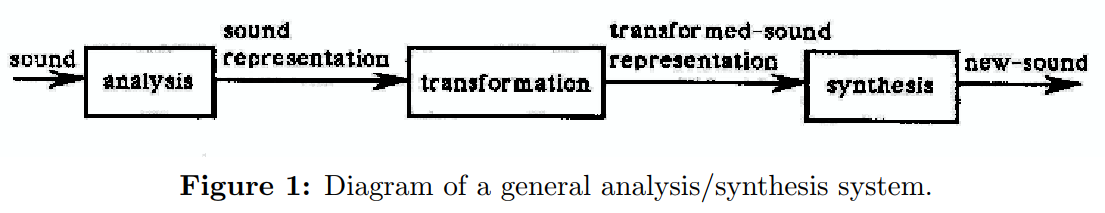
\includegraphics{fig_1.png}
\caption{title}
\end{figure}

    \subsubsection{Background on some Synthesis
Techniques}\label{background-on-some-synthesis-techniques}

    \begin{itemize}
\tightlist
\item
  Historical Background -

  \begin{enumerate}
  \def\labelenumi{\arabic{enumi}.}
  \tightlist
  \item
    Tape Recorders
  \item
    Analog tapes(Music Concrete)
  \item
    Digital
  \end{enumerate}
\item
  Techniques borrowed from Speech Analysis -

  \begin{enumerate}
  \def\labelenumi{\arabic{enumi}.}
  \tightlist
  \item
    Vocoder

    \begin{itemize}
    \tightlist
    \item
      Modeling of speech by an excitation waveform(sound source) which
      is filtered(vocal tract)
    \item
      Were able to obtain interesting sound effects(pitch modification,
      timbre morphing)
    \end{itemize}
  \item
    Linear Predictive Coding

    \begin{itemize}
    \tightlist
    \item
      Linear time varying filtering
    \end{itemize}
  \item
    Phase Vocoder

    \begin{itemize}
    \tightlist
    \item
      Representing signals by the short time phase and amplitude
      spectrum
    \item
      Major motivation to move towards the Short Time Fourier
      Transform(STFT)
    \end{itemize}
  \end{enumerate}
\item
  Synthesis Methods -

  \begin{enumerate}
  \def\labelenumi{\arabic{enumi}.}
  \tightlist
  \item
    LPC based synthesis

    \begin{itemize}
    \tightlist
    \item
      wide variety of transformations because of the decomposition
    \item
      works well when analyzed sounds have \textbf{clear formant
      structure}
    \end{itemize}
  \item
    Analysis based synthesis -

    \begin{enumerate}
    \def\labelenumii{\arabic{enumii}.}
    \tightlist
    \item
      Heterodyne filtering

      \begin{itemize}
      \tightlist
      \item
        breaks input waveform into pseudoperiodic segments and then
        estimates the pitch of each pseudoperiodic segment
      \item
        Similar to STFT, analyzes signal at multiple, evenly-spaced time
        points
      \item
        \href{http://baguyos.tripod.com/DMPST.html}{The Application of
        Heterodyne Filter Analysis and Linear Predictive Coding using
        cSound's ADSYN, LPREAD, and LPRESON Opcodes}
      \end{itemize}
    \item
      Phase Vocoder

      \begin{itemize}
      \tightlist
      \item
        Manipulate Temporal and Spectral Features independently(decouple
        them)
      \end{itemize}
    \item
      Formant wave-function synthesis

      \begin{itemize}
      \tightlist
      \item
        Directly modelling the time domain amplitude
      \item
        \href{https://link.springer.com/chapter/10.1007/978-94-009-9091-3_21}{Time
        Domain FoF}
      \item
        \href{https://ccrma.stanford.edu/~mjolsen/220a/fp.html}{Final
        Project: Formant-Wave-Function Synthesis}
      \end{itemize}
    \item
      VOSIM

      \begin{itemize}
      \tightlist
      \item
        model with sinc pulses of variable amplitudes, delays
      \item
        \href{http://www.atiam.ircam.fr/wp-content/uploads/2011/12/AES_JAES_1978_Kaegi_VOSIM.pdf}{paper}
      \end{itemize}
    \item
      Wavelet transform

      \begin{itemize}
      \tightlist
      \item
        Wavelets as analysis functions
      \end{itemize}
    \end{enumerate}
  \end{enumerate}
\end{itemize}

    \subsubsection{Short Time Fourier
Transform}\label{short-time-fourier-transform}

    \begin{itemize}
\tightlist
\item
  Why perform analysis in the spectral domain?

  \begin{itemize}
  \tightlist
  \item
    Our ear is like a harmonic analyzer, thus spectral analysis mimics
    the bahaviour of the ear
  \item
    Cochlea is likened to a set of narrow band pass filters, thus it
    performs some kind of FT
  \end{itemize}
\item
  How our ear is different?

  \begin{itemize}
  \tightlist
  \item
    Our ear obtains a \textbf{log scale spectrum} as opposed to the
    linear spectra obtained by conventional FT
  \item
    Time and Frequency domain masking
  \item
    Amplitude perception relative to frequency
  \end{itemize}
\item
  \href{http://artsites.ucsc.edu/ems/music/tech_background/te-03/teces_03.html}{Hearing
  and Perception}
\end{itemize}

    The STFT equation -
\(X_{l}(k) := \Sigma_{n=0}^{N-1} w(n)x(n+lH)e^{-j\omega_{k}n}\)

    2 important (controllable) parameters - 1. Analysis window w(n) -
Determines time vs frequency resolution - Want narrow main lobe, low
side lobe - For phase detection, constant phase spectrum obtained by
using symmetric window 2. Hop size H - Depends on sound characteristics

    Why move on? - Cannot manipulate sounds easily

Treat this as an intermediate step to obtain a more flexible
representation

    \subsubsection{Sinusoidal Model}\label{sinusoidal-model}

    Model a signal as a sum of time varying sinusoids\\

\begin{align}
&s(t) = \Sigma_{r=1}^{R} A_{r}(t) cos(\theta_{r}(t))\\
&\theta_{r}(t) = \int_{0}^{t} \omega_{\tau}(\tau)d \tau + \theta_{r}(0) + \phi_{r}
\end{align}

Here, \textbf{R} is the number of sinusoidal components,
\textbf{\(A_{r}(t)\)} is the instantaneous amplitude and
\textbf{\(\theta_{r}(t)\)} is the instantaneous phase

    \begin{figure}
\centering
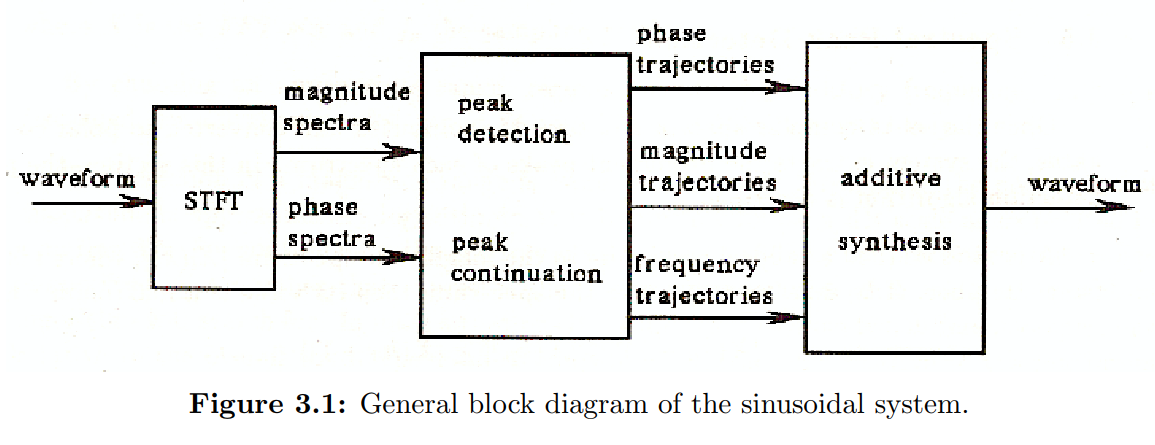
\includegraphics{fig_2.png}
\caption{title}
\end{figure}

    The main steps in the parameter extraction are -

    \begin{enumerate}
\def\labelenumi{\arabic{enumi}.}
\tightlist
\item
  Spectral Peak Detection -

  \begin{itemize}
  \tightlist
  \item
    Peak detection

    \begin{itemize}
    \tightlist
    \item
      Local maxima in the magnitude spectrum at each time frame
    \item
      Filtering the maxima with some threshold measure
    \item
       For perceptual purposes, use knowledge of equal loudness contours
    \end{itemize}
  \item
    Peak interpolation

    \begin{itemize}
    \tightlist
    \item
      Return a better estimate for the frequency than the bin value
    \item
      Fit a parabola to the frequency, and use the peak of parabola as
      estimate The output of this stem is the estimated magnitude,
      frequency and phase of the prominent peaks in the STFT for each
      time frame
    \end{itemize}
  \end{itemize}
\end{enumerate}

    \begin{figure}
\centering
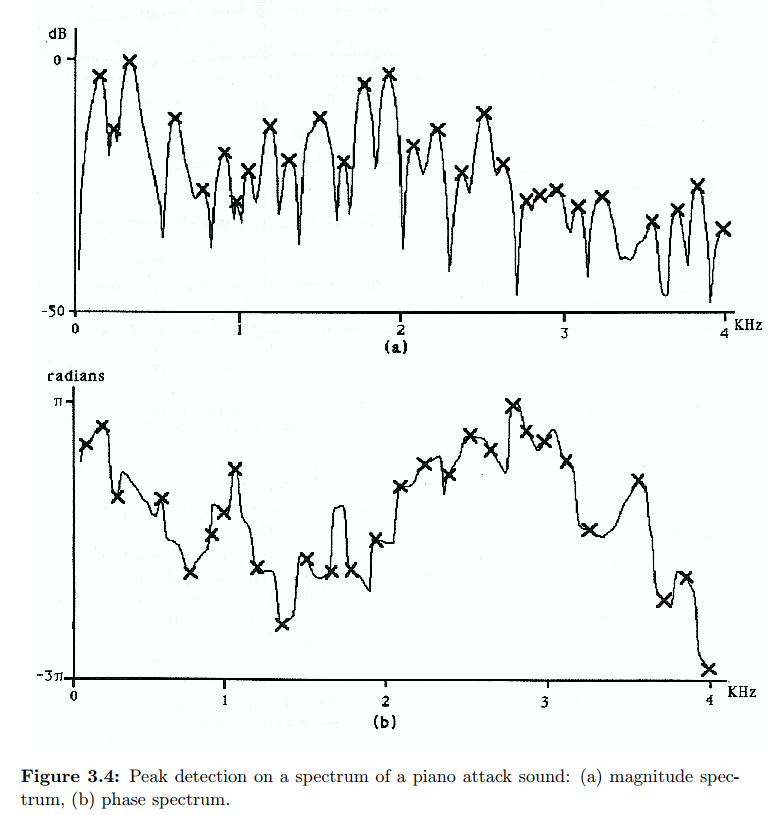
\includegraphics{fig_3.png}
\caption{title}
\end{figure}

    \begin{enumerate}
\def\labelenumi{\arabic{enumi}.}
\setcounter{enumi}{1}
\tightlist
\item
  Spectral Peak Continuation -

  \begin{itemize}
  \tightlist
  \item
    Map the peaks at the \((n-1)^{th}\) time frame to the \((n)^{th}\)
    time frame
  \item
    Find the peak in the \((n)^{th}\) time frame which is closest in
    frequency in the previous frame
  \item
    Possible approaches - heuristic(rule based), probabilistic(hmm)
  \end{itemize}
\end{enumerate}

    \begin{figure}
\centering
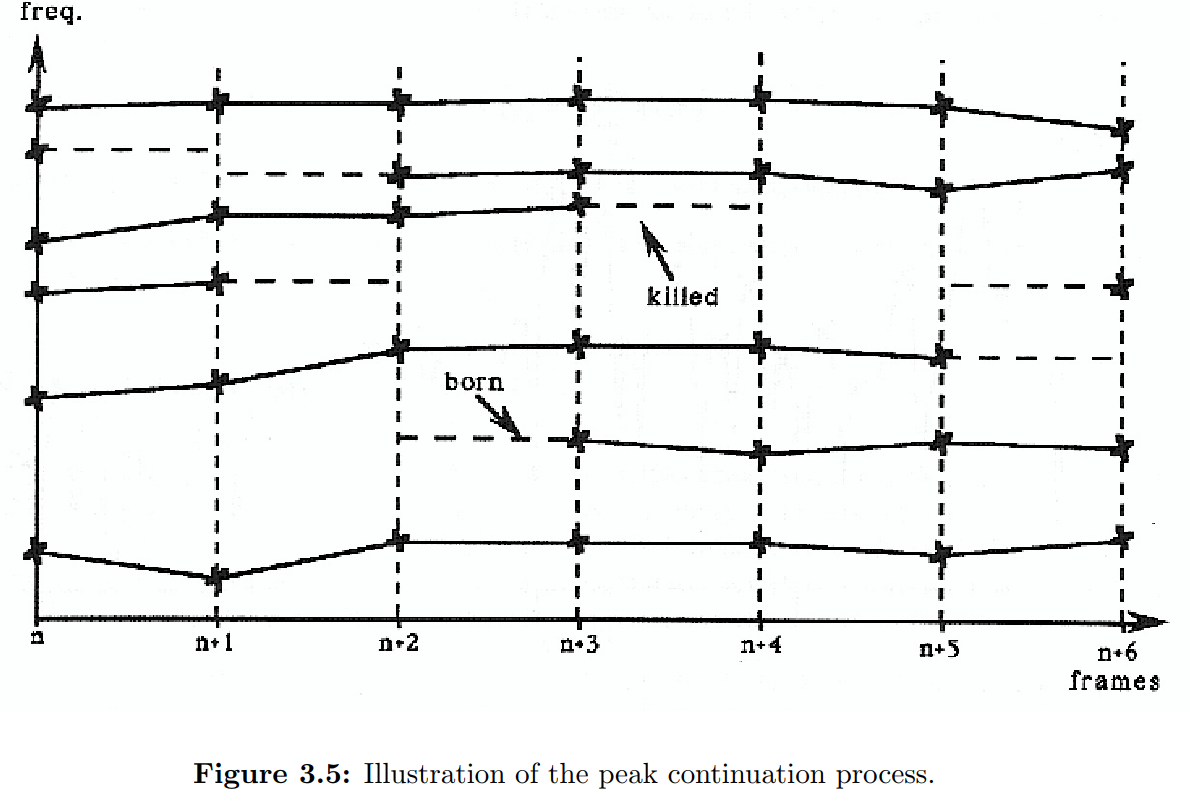
\includegraphics{fig_4.png}
\caption{title}
\end{figure}

    Once the parameters are obtained, the sound is synthesized by generating
the sum of sinusoids for each time frame in the following way -\\

\begin{align}
s^{l}(m) = \Sigma_{r=1}^{R} \hat A^{l}_{r}cos(m\hat \omega^{l}_{r} + \hat \phi^{l}_{r})
\end{align}

    Sound Effects - Can be easily achieved by playing around with the
obtained parameters(scaling, interpolation, filtering etc. ). For ease
of manipulation, only the magnitude spectra is used as the ear is mainly
sensitive to the spectral magnitude and not the phase

    Why move on? - Difficult to model \textbf{noise} with sinsusoids(need a
large number) - Because of the lack of noise modelling, the percieved
quality is a bit artificial during transformations\\
This is motivation to model the noise in the signal as the next step

    \subsubsection{Deterministic + Residual
Model}\label{deterministic-residual-model}

    How is the \textbf{deterministic} component different from the previous?
- As opposed to selecting any peak in the spectrum(like in the previous
case), the deterministic models particularly model the partials in the
sound - Thus, each sinusoid is assumed to model a
\textbf{quasi-sinusoidal} component(piecewise linear amplitude and
frequency variation) as opposed to any kind of sound

The \textbf{Residual} in this case is defined \$ x\_\{original\} -
x\_\{deterministic\} \$. It usually models the energy that does not go
into vibrations, or any component that is not inherently sinusoidal in
nature.

    The signal in this case is modelled as -

\begin{align}
s(t) = \Sigma_{r=1}^{R} A_{r}(t) cos(\theta_{r}(t)) + e(t)\\
\end{align}

Here, e(t) is the residual

    \begin{figure}
\centering
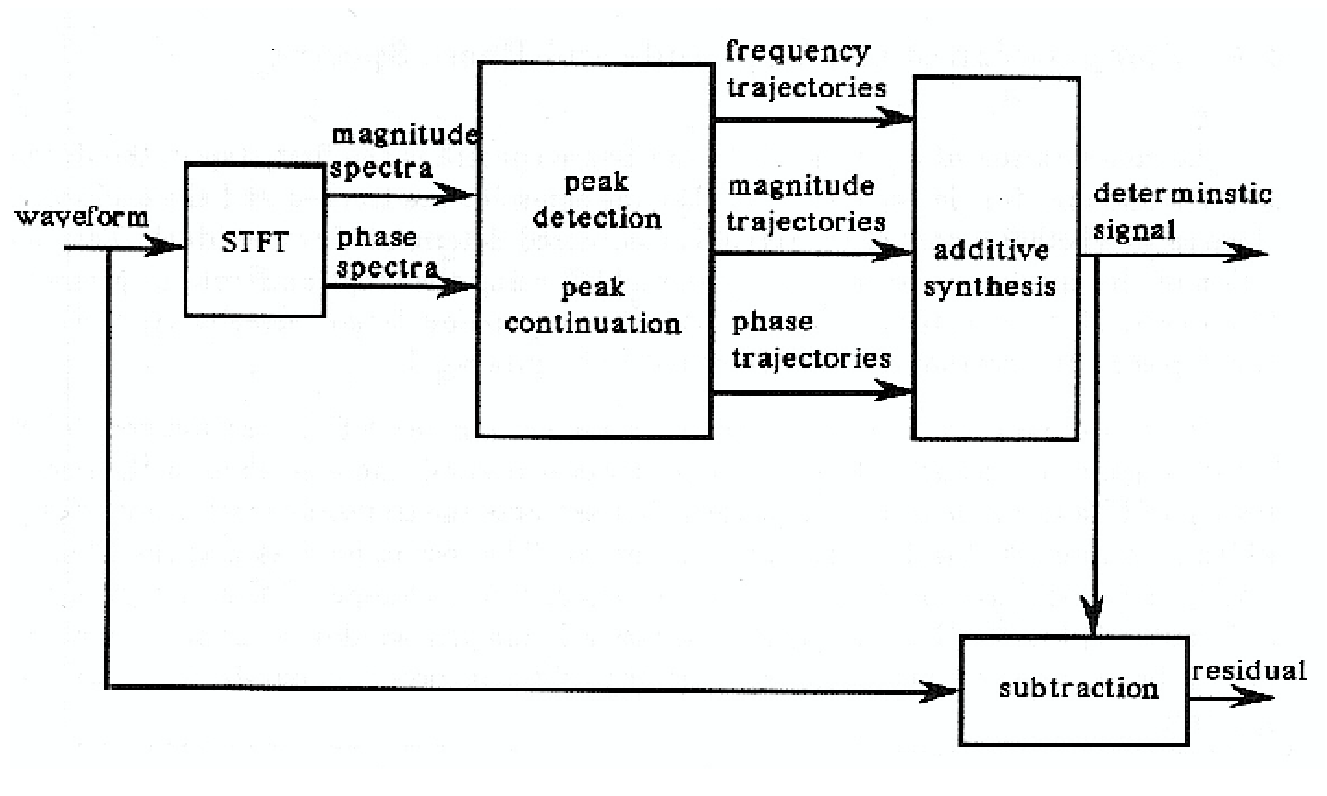
\includegraphics{fig_5.png}
\caption{title}
\end{figure}

    Most of the steps in extracting the parameters for the deterministic
model are the same as the previous model. But, since the sinusoids are
restricted to be partials only here, there is a modification in the
\textbf{Spectral Peak Continuation} process. Using a heuristic(rule
based) and some prior knowledge about the nature of the sound(harmonic,
frequency range etc. ), an algorithm is proposed which tracks only the
clear and stable partials

    The deterministic components are synthesized using the parameters
obtained. The residual is obtained by subtracting this deterministic
signal from the original signal.\\
An easier alternative is to subtract the frequency spectra of the two
signals and ignoring the phase(perceptually unimportant)

    Why move on ? - Residual is not flexible for performing transformations

This motivates to further study the residual, and approximate it with a
model that can be easily played around with.

    \subsubsection{Deterministic + Stochastic
Model}\label{deterministic-stochastic-model}

    Observations from the previous models - - Not necessary to preserve
phase - Can model the residual as some kind of stochastic signal

Modelling the residual as a stochastic signal helps in easily
transforming the signal

\begin{figure}
\centering
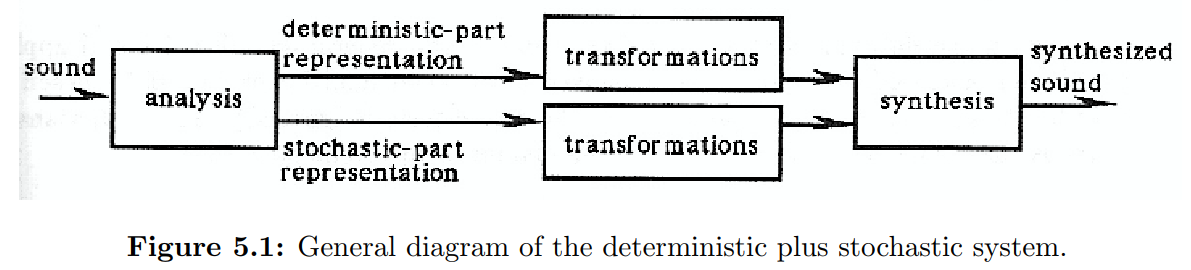
\includegraphics{fig_6.png}
\caption{title}
\end{figure}

    The representation obtained is similar to the previous case, just that
the residual e(t) is modelled as a stochastic signal, thus allowing to
write as the action of a Linear Time Variant system on white noise.\\

\begin{align}
\hat e(t) = \int_{0}^{t}h(t,t-\tau)u(\tau)d \tau
\end{align}

Here, u(t) is white noise and h(t,t') is the filter.

    \begin{figure}
\centering
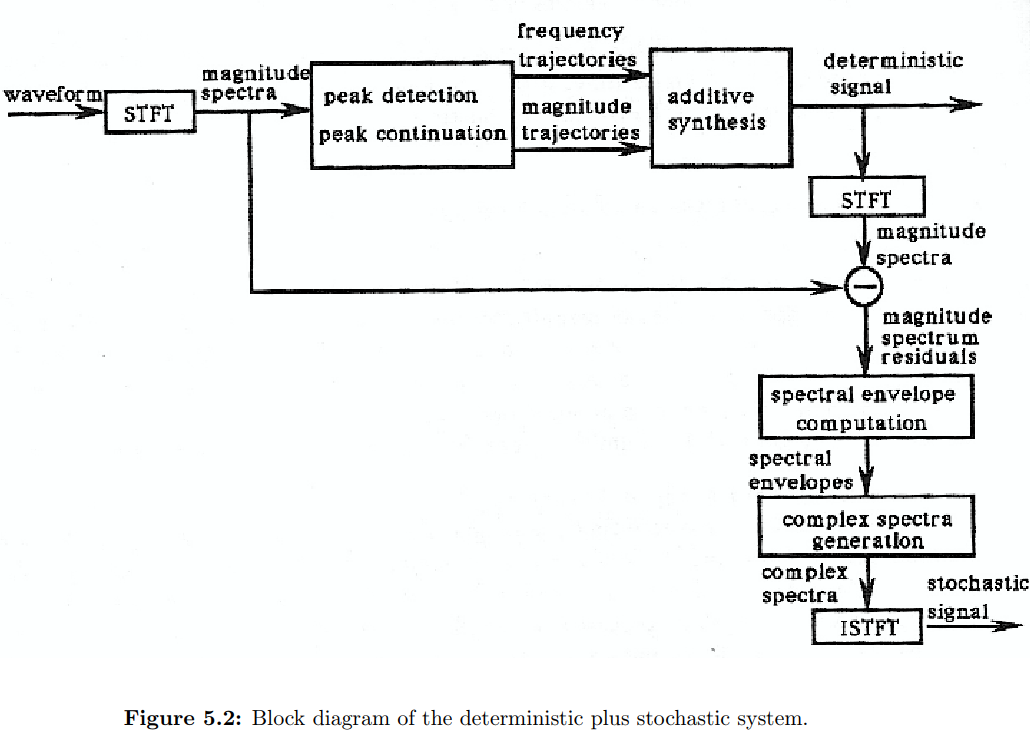
\includegraphics{fig_7.png}
\caption{title}
\end{figure}

    The deterministic component is calculated in the same way as the
previous. The parameters are set in such a way as to extract the
partials as accurately as possible(to prevent them from appearing in the
residual)

    Since we assume the residual to be a stochastic signal, it is
characterized by its amplitude and frequency.\\
To obtain the general shape of the residual spectrum, we approximate the
envelope of the residual spectrum, which is obtained by subracting the
deterministic spectra from the original spectra. This is because only
the shape of the envelope contributes to the sound characteristics. The
envelope is approximated by \textbf{curve fitting} or \textbf{LPC}.\\
Once the envelope is obtained, we generate the stochastic signal by
using this as our amplitude and generate random numbers as phase

\begin{align}
\hat e(t) = IFT(A(k)e^{j \Theta(k)})
\end{align}

Here, A(k) is the envelope, and \(\Theta(k)\) is the phase(random)

    Transformations - Can be separately applied to the deterministic and
stochastic components. - Deterministic - Similar transformations like
before - Stochastic - Envelope shaping, filtering etc.

\begin{figure}
\centering
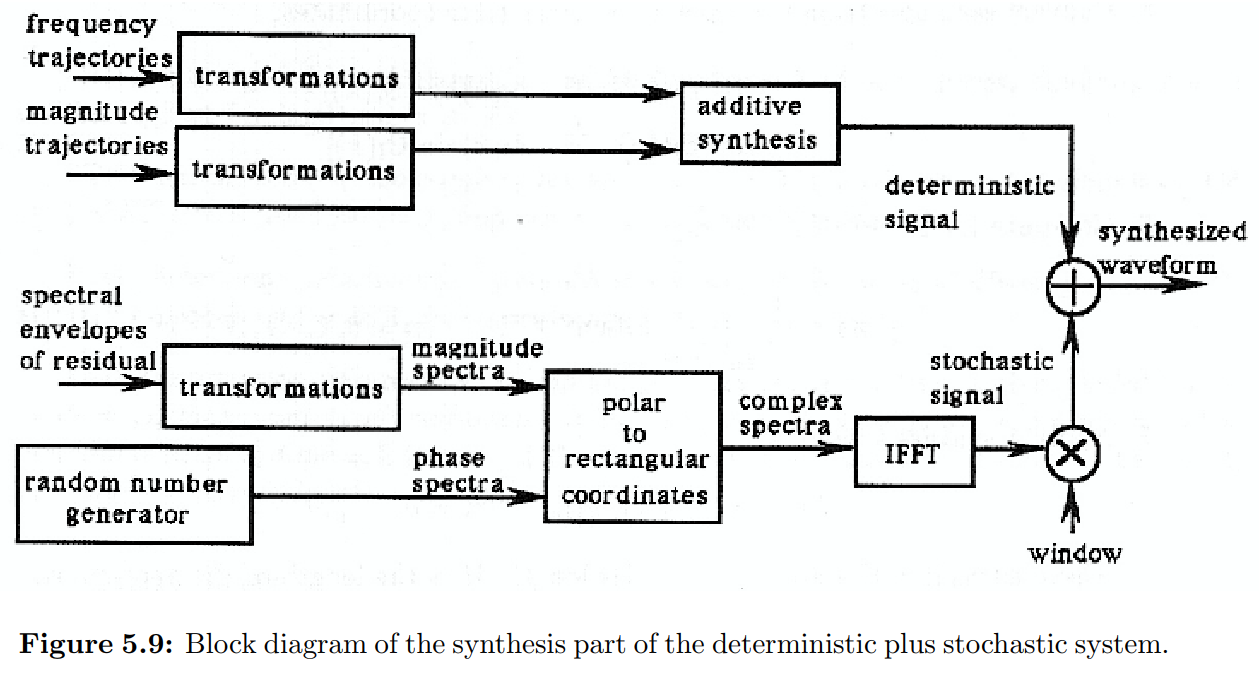
\includegraphics{fig_8.png}
\caption{fig}
\end{figure}

    \subsubsection{Examples of sound effects using the above model (Refer
4.pdf)}\label{examples-of-sound-effects-using-the-above-model-refer-4.pdf}

\begin{enumerate}
\def\labelenumi{\arabic{enumi}.}
\tightlist
\item
  Filtering
\item
  Pitch Scaling, transposition and discretization
\item
  Vibrato, tremolo
\item
  Spectral shape shifting
\item
  Gender changing
\item
  Harmonizing
\item
  Hoarseness
\item
  Morphing
\end{enumerate}

    \begin{center}\rule{0.5\linewidth}{\linethickness}\end{center}

\paragraph{Musical Instrument Sound Morphing Guided by Perceptually
Motivated
Features}\label{musical-instrument-sound-morphing-guided-by-perceptually-motivated-features}

\begin{center}\rule{0.5\linewidth}{\linethickness}\end{center}

For sound examples, visit
\href{http://recherche.ircam.fr/anasyn/caetano/overview.html}{this page}

    What is \textbf{Morphing}?\\
- Blurring Distinction between \textbf{Source} and \textbf{Target} -
Somewhat like creating \textbf{hybrid} musical instruments\\
- Would like to ideally perform \textbf{Perceptually Linear}
transformations - The morphed sound should not simply sound like a
mixture of sounds(the ear can distinguish in such cases). It should
rather sound like a single \textbf{entity}

How is it done?

\begin{itemize}
\tightlist
\item
  Obtain some kind of reprsentation of the sound, and then have an
  interpolation function that gradually interpolates these
  representations from one sound to the other.\\
\item
  Control the whole morphing process(algorithmically and perceptually)
  with a single coefficient \(\alpha\) , the interpolation factor
\item
  You would ideally want to vary the interpolate the parameters so that
  the morphed sound vary \textbf{perceptually linearly}
\end{itemize}

In this work, the authors have proposed to seek sound parameters that
favor Perceptually Linear transformations

    Work done previously\\
- Mostly interpolate parameters/features without caring much about the
perceptual impact 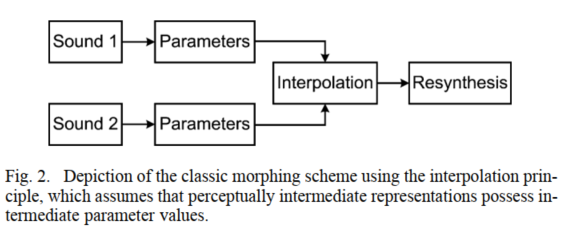
\includegraphics{fig_9.PNG}

What are parameters,features? - Parameters - Coefficients obtained from
sound analysis models(can resynthesize sound from them) - Features -
Particular aspects of sound

Methods Used - 1. Parameter interpolation using Wigner
Distributions(Time Frequency)\\
2. GMM models for parameter interpolation\\
3. \textbf{Model Sounds as dynamical systems with ANN}\\
4. Discrete Wavelet Transform(DWT) + Singular Value Decomposition(SVD)

The above don't consider perceptual factors and suggest suggest
interpolation strategies with better perceptual corelations, like the
ones below 1. Dynamic Frequncy Warping(DFW) to morph spectral envelopes
2. Multi Dimensional Scaling(MDS)

One important thing to consider in all the above cases is the need for
the sound to be \textbf{temporally alligned}, or else some kind of
smearing might occur, thus making the resultant sound artificial to hear

    In this work, as opposed to interpolating parameters directly, the
authors propose to first obtain relevant features from the
parameters(which might have a more perceptual meaning than the
parameters themselves), and then interpolate these features itself.\\
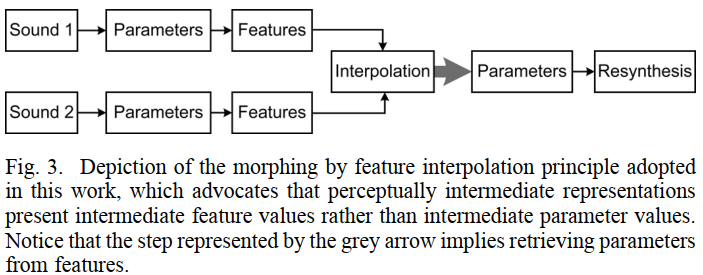
\includegraphics{fig_10.PNG} However, obtaining parameters from features
is difficult(It is not a one-one transformation!). Thus, instead of this
approach, the authors propose to use parameters for whom the
interpolated sounds features are close to the interpolated feature
values(suitable evaluation scheme suggested, use parameters
-\textgreater{} feauture values vary linearly when interpolating
linearly)

    The features the authors use in this work are obtained by finding
\textbf{accoustic correlates of Timbre Spaces using MDS}(Essentially
trying to mathematically describe the Timbre Space). The features are
both temporal and spectral.

Temporal\\
1. log attack time 2. temporal centroid

Spectral 1. spectral centroid 2. spectral spread 3. spectral skewness 4.
spectral kurtosis

The authors proposed model - 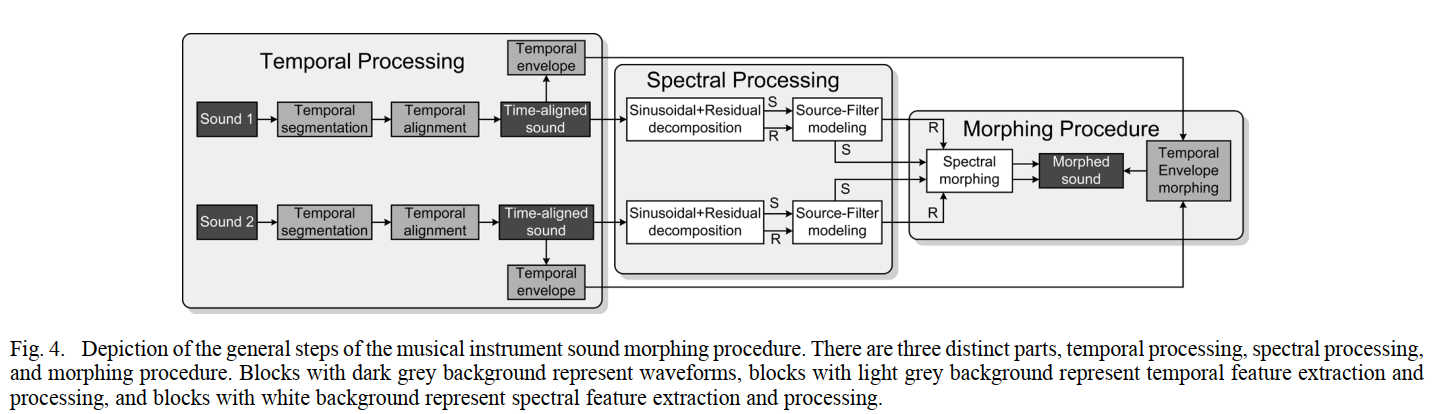
\includegraphics{fig_11.PNG}

    Extraction of Parameter - 1. Temporal Segmentation - Segment into ADSR
2. Temporal Allignment - Boundaries should coincide 3. Temporal Envelope
Extraction - True Amplitude Envelope(TAE) based on cepstral smoothing 4.
Sinusoidal + Residual Model - To obtain the parameters 5. Source Filter
Model -

Morphing - 1. Spectral Envelope Morphing - Shift in frequency peaks
smoothly 2. Interpolation of partial frequencies 3. Temporal Envelope
Morphing

    Evaluation - Vienna Symphonic Library - Listening Test - Judge several
Characteristics for each morph value - Complicated and very subjective -
Proposed Objective error function(assuming linearity, essentially the
MSE)

    \begin{center}\rule{0.5\linewidth}{\linethickness}\end{center}

\paragraph{Spectral Envelope Estimation and Representation for Sound
Analysis--Synthesis}\label{spectral-envelope-estimation-and-representation-for-sound-analysissynthesis}

\begin{center}\rule{0.5\linewidth}{\linethickness}\end{center}

    What is it - Envelope of magnitude of Short Time Spectrum(STS) 1. Speak
about \textbf{Spectral Envelopes} in sound analysis and synthesis. 2.
Linked to perception, and how they capture \textbf{important properties}
of sound. 3. Challenges - Not east to estimate and represent them

    What you want - 1. Envelope fit - Links the peaks of partials 2.
Smoothness - should not oscillate wildly, just give a rough idea of the
shape 3. Adaptation to fast spectral variations

    Methods of Estimation - 1. Linear predictive coding 2. Cepstrum 3.
Discrete cepstrum

What is wanted - 1. Precision 2. Stability(like BIBO, small changes in
data should give small changes in output) 3. Locality in frequency -
parameters should cause local, not global changes 4. Flexibility and
ease of manipulations - Should be easily manipulable with tunable
parameters 5. Speed of synthesis 6. Space in memory 7. Manual input -
manual tuning/control

Proposed Representations - 1. Filter coefficients 2. Sampled
representation 3. Geomteric representation 4. Formants

    What can be done with them - 1. Influence timbre 2. Enhance musical
expressivity

Link to webpage describing the above in detail -
\href{http://recherche.ircam.fr/anasyn/schwarz/publications/icmc1999/se99-poster.html}{link}

    \begin{center}\rule{0.5\linewidth}{\linethickness}\end{center}

\paragraph{AUTOMATIC TIMBRAL MORPHING OF MUSICAL INSTRUMENT SOUNDS BY
HIGH-LEVEL
DESCRIPTORS}\label{automatic-timbral-morphing-of-musical-instrument-sounds-by-high-level-descriptors}

\begin{center}\rule{0.5\linewidth}{\linethickness}\end{center}

    Precursor to the second paper above.\\
Speak about the importance of taking into account perception while
morphing(go through paper highlights, most work is extension of 2

    \begin{center}\rule{0.5\linewidth}{\linethickness}\end{center}

\paragraph{AUTOMATIC AUDIO MORPHING}\label{automatic-audio-morphing}

\begin{center}\rule{0.5\linewidth}{\linethickness}\end{center}

    Automatic morphing from one sound to another - Sound represented in a
multi-dimensional space - Axes represent features that
\textbf{perceptually represent} the sound, in this case spectral shape
and pitch - The axes are assumed to be orthogonal i.e. each axis can be
transformed independent of the others - Morphing essentially represents
interpolation in this space

    One sound should \textbf{smoothly} change into another sound. The
process is described below in the figure - 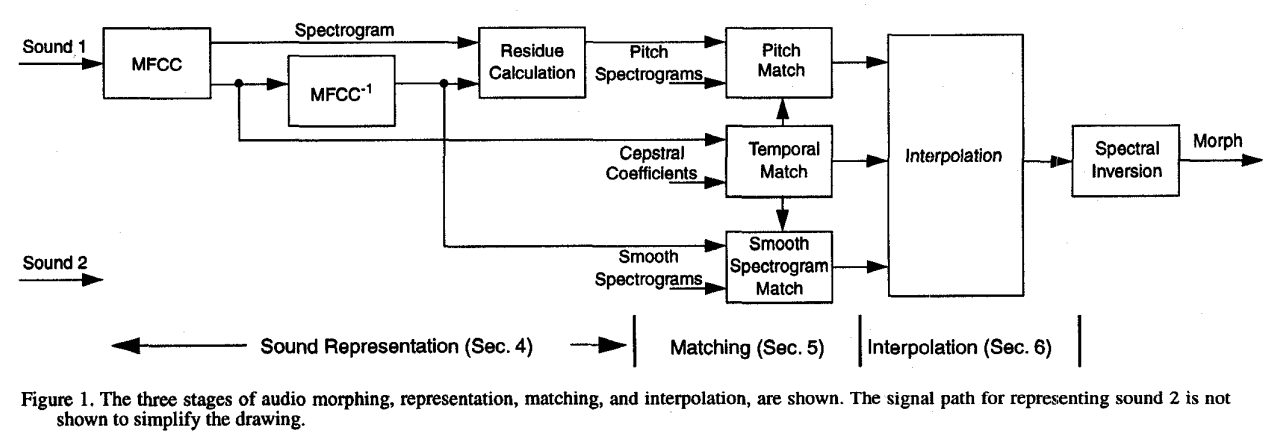
\includegraphics{fig_12.PNG}
1. A sound representation in the 'space'(in this case pitch and
envelope) is obtained. 2. Matching(allignment) to allign relevant
features 3. Interpolation, followed by reconstruction

Spectrograms are used to encode the two axes(smooth spectrogram using
MFCC's, followed by a pitch spectrogram)

    The morphing - Linear interpolation between the matched features
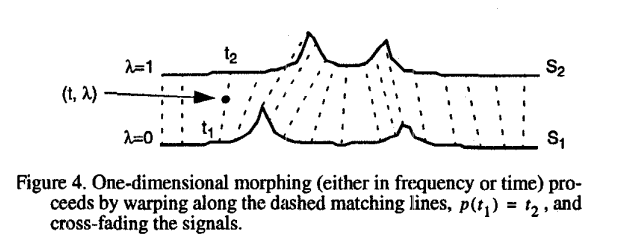
\includegraphics{fig_13.PNG} The signal is linearly interpolated in time
from features of signal 1 to signal 2.

    Future work - 1. Better repesentations 2. Better matching techniques 3.
\textbf{Perceptually optimal interpolation functions}

    \begin{center}\rule{0.5\linewidth}{\linethickness}\end{center}

\paragraph{Creative Music(Work by Tristan Jehan at MIT Media
Lab)}\label{creative-musicwork-by-tristan-jehan-at-mit-media-lab}

\begin{center}\rule{0.5\linewidth}{\linethickness}\end{center}

    What has he done - In his Masters thesis\textless{}11\textgreater{}, He
has made what he calls a \textbf{hyperviolin} - An instrument whose
sounds/timbre can be modified in realtime by modifiying parameters.
Then, in his PhD thesis\textless{}10\textgreater{}, he creates a system
which can basically \textbf{create} music from data.

    \begin{center}\rule{0.5\linewidth}{\linethickness}\end{center}

Msc Thesis - Audio Driven Timbre Generator Salient points - -
\textbf{Little to no digital synthesis technology for non keyboard
instruments}\{Potential Work area\} - Limitations in current systems are
- 1. Quality 2. Control over synthesis 3. Instrument specific -
Hyperviolin - 1. Takes musical performance data(audio + gesture) 2.
Processing(can be in realtime) 3. Generation/Synthesis - They model
\textbf{Physical Sound}, not the perceptual features(What they call
\textbf{Timbre Model}) - \textbf{Almost no work done on
perceptually-controlled sound synthesis}\{Potential Work area\} - Future
work - 1. Algorithms that extract \textbf{better and new} perceptual
features 2. Study the \textbf{evolution of parameters} rather than
instantaneuos parameters i.e. take into account how parameters evolve in
the piece and transform accordingly

    \begin{center}\rule{0.5\linewidth}{\linethickness}\end{center}

PhD Thesis - Creating Music by Listening - High degree of abstraction
between sampled audio and mental perception of it. Authors propose to
bridge this gap by modeling human perception and learning of music. -
Composing new music by \textbf{recycling} pre-existing music. - Thinks
of all possible audio signals as a space. Music is a very small subset
with some structure in this space. The authors want to make an
\textbf{intelligent search} in this space to \textbf{re-discover} music.

    Interesting points - - Perceptual Synthesis Engine(MSc thesis work, SMS
+ Perception) -\textgreater{} Decompose audio to parameters(frequency,
amplitude) and their perceptual correlates(instantaneuos pitch,
loudness, brightness), then learn relation between two data - Use other
metadata(besides audio) like acoustic, cultural editorial for
retrieval\{Can we do for synthesis, study what kinds of metadata is
available\}

    \textbf{Music Cognition Machine} 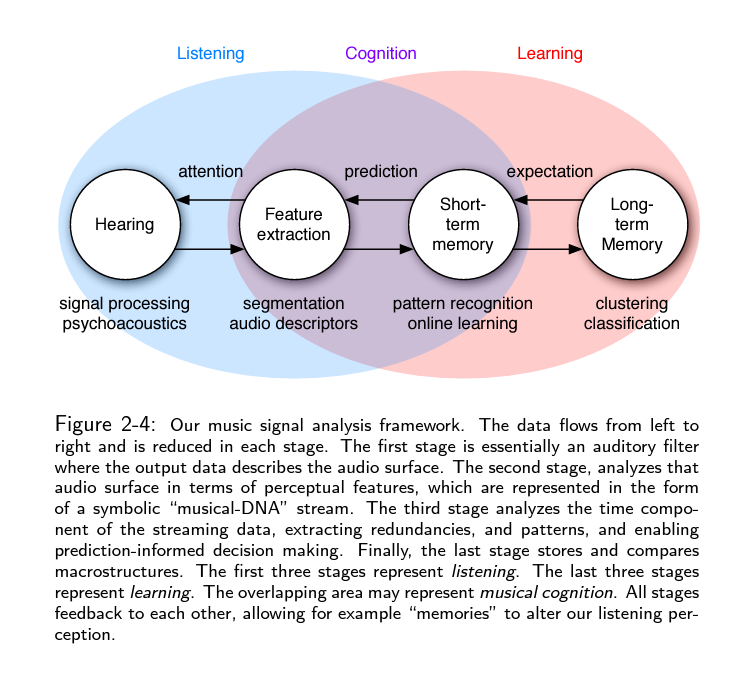
\includegraphics{fig_14.PNG}


    % Add a bibliography block to the postdoc
    
    
    
    \end{document}
